\subsection{Recherche}
Anfangs hatte ich Schwierigkeiten, die Zeit zu finden, mich mit der Codebasis des Realtime Football Analysis Tools vertraut zu machen, daher konzentrierte ich mich auf andere Aufgaben im Projekt. Die naheliegendste Entscheidung war die Recherche, um Informationen zu sammeln, auf die sich die Arbeit anderer Teammitglieder stützen konnte.

\subsubsection{Flask Recherche}
Als Erstes habe ich die Flask-Manpages nach allen für unser Projekt relevanten Seiten gefiltert. Da die Flask-Dokumentation recht umfangreich ist, habe ich hierfür ChatGPT verwendet. Zugegeben, hier ist keine nennenswerte Arbeit meinerseits zu sehen, aber ich wollte sie trotzdem einfügen, da sie zukünftige Recherchen zu Flask erleichtern könnte. Das Ergebnis der harten Arbeit von ChatGPT befindet sich im Projektordner und trägt den Namen „flask\_imports\_doc.txt“.

\subsubsection{Recherche für den NCAA Strafenkatalog}
Ein Ziel dieser Projektgruppe war die Erweiterung der Möglichkeiten des Realtime Football Analysis Tools zur Erfassung von Strafen und deren Konsequenzen. Dazu recherchierte ich alle möglichen Strafen der National Football League (NFL) und fasste sie in einem Dokument zusammen. Dabei wurde mir klar, dass die deutschen Football-Regeln nicht auf dem Regelwerk der NFL, sondern auf dem detaillierteren und den Spielern gegenüber weniger gefährlichen Regelwerk der National Collegiate Athletic Association (NCAA) basieren. Um dies zu korrigieren, mussten einige Regeln angepasst und viele kleine Regeln hinzugefügt werden. Im Großen und Ganzen sind sich beide Regelwerke jedoch sehr ähnlich. Die vollständige Ausarbeitung kann im Projektordner unter dem Namen „Football Penalty Recherche NCAA.txt" gefunden werden.

\pagebreak

\subsection{Programmieren}
Diese Sektion gibt einen Überblick über meine Programmierarbeit an dem Realtime Football Analysis Tool. Ich nahm die Codeschnipsel, die meine Arbeit darstellen aus der git diff, da dort schön gezeigt wird was dazugekommen ist und was verschwand. Außerdem kann man aus der Überschrift die Zeilennummer herauslesen.
\subsubsection{Play Type in Drive List anzeigen}
Das Problem mit der aktuellen Game Page bestand darin, dass die Drives nicht ihren Play Type anzeigten. Dadurch war es ziemlich schwierig, den Überblick darüber zu behalten, wer im Moment im Besitz des Drives ist. Meine einfache Lösung bestand darin, den Play Type bei jedem Eintrag in der Drive List anzuzeigen. Das Endergebnis ist unten dargestellt.
\\ \\
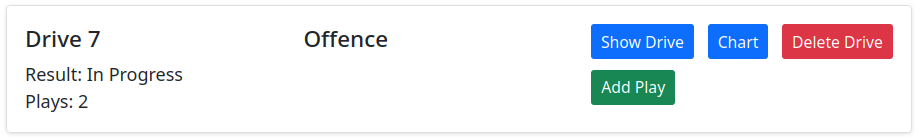
\includegraphics[width=\textwidth]{Drive_list_button.png} \\

Damit der Play Type in der Drive List angezeigt wird, schicken wir zunächst eine query an die Datenbank und speichern die Drive Id in der 'drive' Variable:

\begin{minted}{python}
	@@ -31,7 +31,7 @@ class PlayController:
	
	options = self._get_add_play_form_options()
	play = PlayModel.query.get_or_404(play_id)
	-
	+       	drive = DriveModel.query.get_or_404(play.drive_id)
	if request.method == 'POST':
	try:
	result_form = request.form.get('result')
\end{minted}


Daraufhin iterieren wir durch die drives um festzustellen ob sie leer sind oder schon Plays darin eingetragen sind und geben wenn ja wir für jeden drive den 'odk' Entry des ersten Plays aus, einfachheitshalber:

\begin{minted}{python}
@@ -66,6 +66,9 @@ class GameController:
	
	@login_required
	def game_detail(self, game_id: int) -> str:
		game = GameModel.get_by_id(game_id)
+       for drive in game.drives:
+            if len(drive.plays) > 0:
+                print(drive.plays[0].odk)
		return render_template(template_name_or_list='game/game_detail.html', game=game)
\end{minted}

Noch eine Sache ist im Controller zu erledigen: wir müssen dem HTML template the Drive Id übergeben.

\begin{minted}{python}
@@ -67,6 +67,7 @@ class PlayController:
        return render_template('play/add_play.html',
                                play=play,
+                               drive=drive,
                                options=options,
                                drive_id=play.drive_id)
\end{minted}

Nun zum interessanten Teil: Die HTML-Vorlage soll den Play Type in jedem Feld der Drives auf der Game Page darstellen. Der folgende Code zeigt den Spieltyp entweder als „Offence“, „Defence“ oder „Special“ an, wenn der Datenbankeintrag für den ersten Spieltyp entweder „O“, „D“ oder „K“ lautet. Der angegebene Text wird als Kartentitel nach dem Drive-Name platziert.

\begin{minted}{html}
@@ -41,6 +41,18 @@
			<div class="card-body">
				<div class="d-flex justify-content-between align-items-start">
				<h5 class="card-title">Drive {{ loop.revindex }}</h5>
+                
+                    
+                        <h5 class="card-title">Offence</h5>
+                    
+                        <h5 class="card-title">Defence</h5>
+                    
+                        <h5 class="card-title">Special</h5>
+                    
+                        <h5 class="card-title">Unknown play type: {{ drive.plays[0].odk }}</h5>
+                    
+
+                

					<div>
						<a href="{{ url_for('drive_play_chart', game_id=game.id, drive_id=drive.id) }}" class="btn btn-sm btn-primary">Chart</a>	
\end{minted}

\subsubsection{Add Play Knopf in der Drive List}
Mein nächster Story Point war die Integration des 'Add Play' Buttons in dem Panel des Drive List Eintrags, ein Gebiet, mit dem ich bereits aus dem letzten Kapitel vertraut war. Der 'Add Play' Button wurde bereits im letzten Absatz gezeigt, aber hier ist er noch einmal:
\\ \\
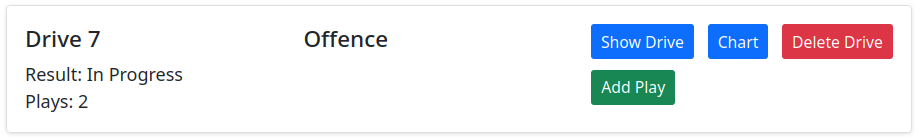
\includegraphics[width=\textwidth]{Drive_list_button.png} \\

Ich entscheid mich dazu dem Add Play Button unter die anderen Knöpfe des Drive Panels zu setzen, da die Funktion mir separat von den drei anderen Knöpfen erschien. Unten ist die '\_drive\_rows.html abgebildet, der ich nach dem 'Result: ' Eintrag den Add Play Button eingefügt und mit einer Margin manuell zur Mitte orientiert habe:
\begin{minted}{html}
@@ -31,12 +37,16 @@
						
						<button class="btn btn-sm btn-secondary" disabled>Delete Drive</button>
						
+                        
+                   </div>
+               </div>
+               <div class="d-flex justify-content-between align-items-center">
+                   <div class="card-text mb-0">
+                        Result: {{ drive.result or 'In Progress' }}<br>
+                        Plays: {{ drive.plays|length }}
					</div>
+                   <a href="{{ url_for('add_play', drive_id=drive.id) }}" class="btn btn-sm btn-success ms-auto" style="margin-right: 12.1rem;">Add Play</a>
				</div>
-               <p class="card-text">
-                   Result: {{ drive.result or 'In Progress' }}<br>
-                   Plays: {{ drive.plays|length }}
-                </p>
			</div>
		</div>
\end{minted}

Ich beschloss die 'Show Drive' und 'Cart' Knöpfe zu vertauschen und das hatte zwei Gründe: \\
Erstens wäre der 'Chart' Button kleiner als der 'Add Play' Button, was im Layout sehr unangenehm aussehen würde, da die beiden Knöpfe sich in ihrer vertikalen Platzierung überlappen würden. \\
Zweitens mach es mehr Sinn für den 'Show Drive' Knopf vorne zu sein, da es der Knopf ist, den man am meisten benutzt. 
Außerdem passte ich die Position der genannten Knöpfe ebenfalls mit Margins an, um den Abstand zwischen ihnen gleichmäßig zu halten.

\begin{minted}{html}
@@ -19,10 +19,16 @@
	<div>
-		<a href="{{ url_for('drive_play_chart', game_id=game.id, drive_id=drive.id) }}" class="btn btn-sm btn-primary">Chart</a>
-                        
+ 		<a href="{{ url_for('drive_detail', drive_id=drive.id) }}" class="btn btn-sm btn-primary">Show Drive</a>
+                        
+		<a href="{{ url_for('drive_play_chart', game_id=game.id, drive_id=drive.id) }}" class="btn btn-sm btn-primary", style="margin-right: 0.5rem;">Chart</a>
\end{minted}

Daraufhin hatte ich die Idee alle Knöpfe im Realtime Football Analysis Tool die etwas erstellen grün zu färben, um das Layout des Programms einheitlich zu halten. Unten sieht man ein Beispiel dafür, aber es ist nicht die einzige Instanz:

\begin{minted}{html}
-                <a href="{{ url_for('add_play', drive_id=drive.id) }}" class="btn btn-primary">Add Play</a>
+                <a href="{{ url_for('add_play', drive_id=drive.id) }}" class="btn btn-success">Add Play</a>
\end{minted}


\subsubsection{Kleine Angelegenheiten}
Der folgende Code ist eine kleine Anpassung beim Datum im Titel der Drive List. Es soll das vertraute Punktesystem zusammen mit dem gut lesbaren DDMMYYYY Format kombinieren:
\begin{minted}{html}
@@ -4,8 +4,8 @@
 
 <div class="row mb-4">
	<div class="col">
-        <h2>{{ game.game_name }}</h2>
-        <p>{{ game.date.strftime('%Y-%m-%d') }} {{ game.time }}</p>
+        <h2>{{ game.name }}</h2>
+        <p>{{ game.date.strftime('%d.%m.%Y') }} {{ game.time }}</p>
	</div>
\end{minted}

Außerdem habe ich hier meinen ersten Bug gefunden. Der Variablenname game.game\_name löste aus, dass der Titel des Games über der Drive List nicht richtig angezeigt wurde. Der Name game.name war richtig und vervollständigte den Titel wieder.

\pagebreak

\subsection{Design des Namens und des Logos}
Meine letzte Aufgabe war die Erfindung eines neuen Namens und das Design eines neuen Logos passend dazu.

\subsubsection{Name}
Ich wollte ich dem Realtime Football Analysis Tool einen Namen geben der in sich eine Abkürzung für eine grobe Beschreibung der Funktion ergibt, wie viele Programme und Konzepte ihn heute besitzen. Beispiele dafür sind GIMP, SCRUM oder das GNU-Projekt. Meine Inspiration dazu kam tatsächlich von dem alten Namen, aber die Abkürzung RFAT war unsinnig und rollte nicht von der Zunge wenn man sie aussprach. Ich ging daraufhin einige Fachbegriffe des American Football durch und versuchte sinnvolle Worte für jeden Buchstaben zu finden. \\
Letztendlich entschied ich für Simple Number Analysis Platform (SNAP), das den Moment des Anpfiffs eines Plays als Namen verwendet. Für den Fall, das einem zukünftigen Entwickler der Name nicht gefällt liefere ich hiermit noch zwei Alternativen: \\
Data-Driven Realtime Insights and Visual Evaluation (DRIVE) und \\
Realtime Unified Statistical Hub (RUSH).

\subsubsection{Logo}

\begin{wrapfigure}{r}{175px}
	\vspace{-10pt}
	\hspace{15pt}
	
\includegraphics[width=150px]{logo.png}
\end{wrapfigure}

Das Logo sollte den Namen des Programms verdeutlichen, was hier mit einem Football dargestellt wird der von einer Hand auf ein Footballfeld gestellt wird, wie es in dem Moment des Snaps geschieht.
Das Logo wurde rein mit LibreOffice Draw erstellt und mit GIMP ein Alpha Kanal hinzugefügt. Das Logo ist im Login und im Symbol des Tabs von SNAP zu sehen. 